% !TeX program = lualatex
% !TeX encoding = utf8
% !TeX spellcheck = uk_UA
% !BIB program = bibler

\documentclass{beamer}
\usetheme{Electromagnetism}
\usepackage{Electromagnetism}


%============================================================================
\title[Лекції електрики та магнетизму]{\huge\bfseries Система рівнянь Максвелла}
\subtitle{Лекції з електрики та магнетизму}
\author{Пономаренко С. М.}
%============================================================================
\graphicspath{{pictures/}}
\begin{document}
\begin{frame}[plain]
	\maketitle
\end{frame}

% ============================== Слайд ## ===================================
\begin{frame}{Зміст}{}
	\tableofcontents
\end{frame}
% ===========================================================================




% ============================== Слайд ## ===================================
\begin{frame}{Основоположники теорії електромагнітного поля}{}
	\begin{block}{}\justifying
		Теорія електромагнітного поля, початки якої заклав \alert{Фарадей}, математично була завершена \alert{Максвеллом}. При цьому однією з найважливіших
		нових ідей, висунутих Максвеллом, була думка про симетрію в взаємозалежності електричного і магнітного полів.
	\end{block}

	\begin{tblr}{
		colspec={X[c,m]X[c,m]},
		row{2} = {c,m, font=\scriptsize}
		}
		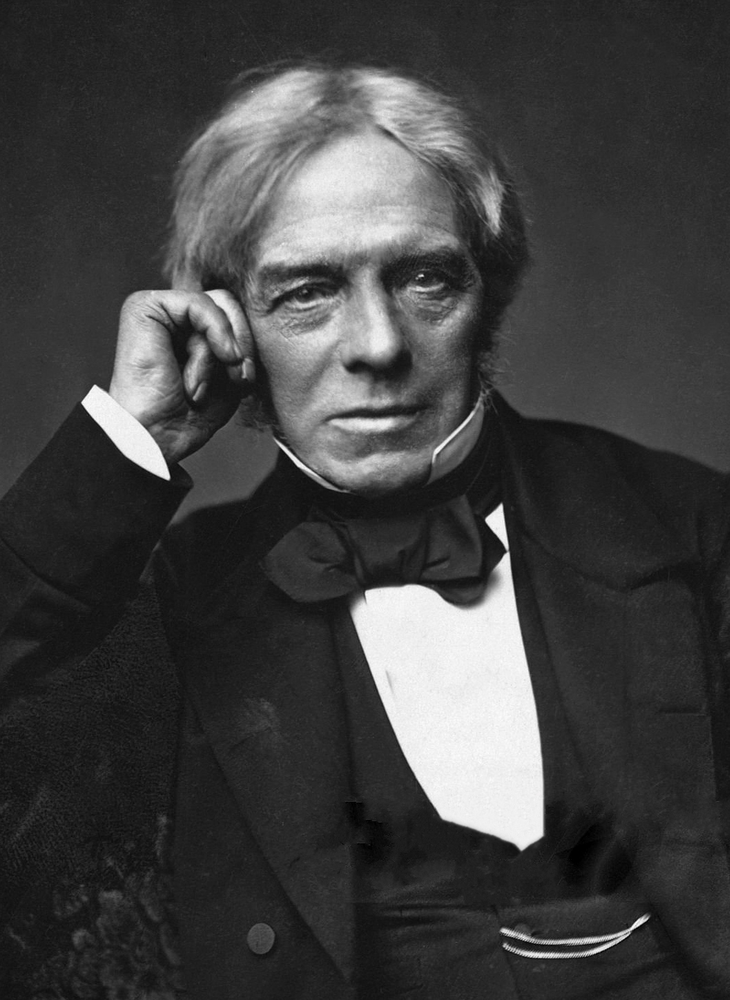
\includegraphics[height=0.75\linewidth]{Faraday} & 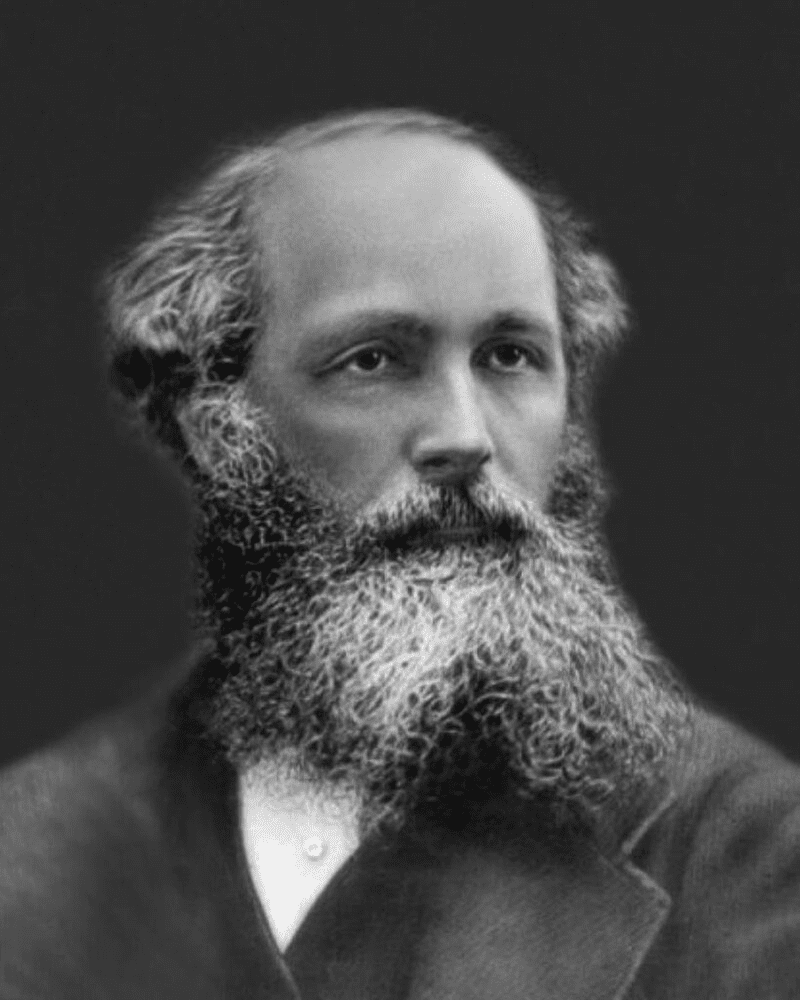
\includegraphics[height=0.75\linewidth]{Maxwell} \\
		\href{https://en.wikipedia.org/wiki/Michael_Faraday}{Майкл Фарадей} (1791 -- 1867) --- англійський фізик і хімік.
		                                                 &
		\href{https://en.wikipedia.org/wiki/James_Clerk_Maxwell}{Джеймс Клерк Максвелл} (1831 -- 1879) --- шотландський вчений.
	\end{tblr}
\end{frame}
% ===========================================================================

% ============================== Слайд ## ===================================
\begin{frame}{Цитати із книги <<Еволюція фізики>>}{А. Ейнштейн, Л. Інфельд}
	\begin{block}{}\justifying
		Кількісне, математичне формулювання законів поля дано в так званих рівняннях Максвелла. [Експериментальні] факти призвели до формулювання цих рівнянь,
		але зміст їх значно багатший [\ldots]. Їхня проста форма приховує глибину, що виявляється тільки при ретельному вивченні.

		\bigskip

		Формулювання цих рівнянь є найважливішою подією з часу Ньютона не тільки важливою подією з часу Ньютона не тільки внаслідок цінності їхнього змісту, а й
		тому, що вони дають зразок нового типу законів. Характерну особливість рівнянь Максвелла, яка проявляється і в усіх інших рівняннях сучасної фізики,
		можна виразити в одному реченні: \alert{рівняння Максвелла суть закони, що виражають структуру поля}.
	\end{block}
\end{frame}
%

%% --------------------------------------------------------
\section{Струм зміщення}
%% --------------------------------------------------------===========================================================================

% ============================== Слайд ## ===================================
\begin{frame}{Струм зміщення і закон збереження заряду}
	\framesubtitle<1>{Протиріччя в законах магнетизму}
	\begin{onlyenv}<1>
		\begin{block}{}\justifying
			Теорема про циркуляцію для постійного магнітного поля:
			\begin{equation*}
				\Rot\Hfield = \frac{4\pi}{c}\vect{j}
			\end{equation*}
			виявляється невірною у випадку змінного електричного поля.

			\bigskip

			Застосовуючи операцію $\Div$ до цього рівняння і
			враховуючи тотожність $\Div\Rot\Hfield = 0$, отримуємо $\Div\vect{j} = 0$. З іншого
			боку, якщо густина заряду змінюється з часом, $\frac{\partial\rho}{\partial t} \neq 0$ то в силу
			закону збереження заряду
			\begin{equation*}
				\Div\vect{j} = - \frac{\partial\rho}{\partial t},
			\end{equation*}
			тобто $\Div\vect{j} \neq 0$. Це протиріччя показує, що необхідно
			видозмінити теорему про циркуляцію.
		\end{block}
	\end{onlyenv}
	\framesubtitle<2>{Гіпотеза Максвелла}
	\begin{onlyenv}<2>
		\begin{block}{}\justifying
			Для вирішення цього протиріччя Дж. Максвелл увів поняття \alert{струму зміщення} $\vect{j}_\text{зм}$ співвідношенням
			\begin{equation*}
				\Rot\Hfield = \frac{4\pi}{c}(\vect{j} + \vect{j}_\text{зм}),
			\end{equation*}
			щоб закон збереження заряду виконувалося. Застосовуючи операцію $\Div$ до записаного рівняння,
			отримуємо:
			\begin{equation*}
				\Div(\vect{j} + \vect{j}_\text{зм}) = 0, \ \Rightarrow\ \Div\vect{j}_\text{зм} = \frac{\partial\rho}{\partial t}.
			\end{equation*}
			За теоремою Гаусса для електричного поля $\rho = \frac1{4\pi}\Div\Dfield$. Отже:
			\begin{equation*}
				\Div\vect{j}_\text{зм} = \frac{\partial}{\partial t}\left( \frac1{4\pi}\Div\Dfield \right),\ \Rightarrow\ \tcbhighmath{\vect{j}_\text{зм} =
					\frac1{4\pi}\frac{\partial\Dfield}{\partial t}.}
			\end{equation*}
		\end{block}
	\end{onlyenv}
	\framesubtitle<3>{Теорема про циркуляцію магнітного поля}
	\begin{onlyenv}<3>
		\begin{block}{}\justifying
			Таким чином, теорема про циркуляцію для магнітного поля,
			що узгоджується із законом збереження заряду, має записуватися у вигляді
			\begin{equation*}
				\tcbhighmath{\Rot\Hfield = \frac{4\pi}{c}\vect{j} + \frac1c\frac{\partial\Dfield}{\partial t},}
			\end{equation*}
			В інтегральній формі теорема про циркуляцію має вигляд
			\begin{equation*}
				\oint\limits_L \Hfield\cdot d\vect{r} = \frac{4\pi}{c} \iint\limits_S\vect{j}\cdot d\vect{S} + \frac1c\iint\limits_S
				\frac{\partial\Dfield}{\partial t} \cdot d\vect{S},
			\end{equation*}
			де $I_\text{зм} =  \frac1{4\pi} \iint\limits_S\frac{\partial\Dfield}{\partial t} \cdot d\vect{S}$ --- струм зміщення, що пронизує площу $S$, натягнуту
			на контур $L$.
			Отже, згідно гіпотези Максвелла \alert{змінне електричне поле поряд зі звичайними струмами, також створює магнітне поле}.
		\end{block}
	\end{onlyenv}
	\framesubtitle<4>{Порівняння закону Фарадея та гіпотези Максвелла}
	\begin{onlyenv}<4>
		\begin{block}{}\justifying
			Порівняємо закон електромагнітної індукції Фарадея, та <<оновлену>> теорему про циркуляцію за відсутності струмів провідності ($\vect{j} = 0$) у
			вакуумі ($\epsilon = \mu = 1$ $\Rightarrow$ $\Efield = \Dfield$, $\Hfield = \Bfield$).
			\begin{center}
				\begin{tblr}%
					{
					colspec={X[c,m]X[c,m]},
					row{2}={c,m,mode=dmath},
					}
					Закон електромагнітної індукції                          & Закон магнітоелектричної індукції                        \\
					\Rot\Efield = -\frac1c\frac{\partial\Bfield}{\partial t} & \Rot\Bfield = +\frac1c\frac{\partial\Efield}{\partial t} \\
					\tikz[rotate=90, scale=0.9, >=latex, midarrow/.style={%
								postaction={ decorate,
										decoration={ markings, mark=at position .7 with {\arrow{latex}}}}}]{
						\begin{scope}[xshift=0.25cm]
							\draw[arrowpos={0.5}{2pt}{4pt}, red] (1.1,0) [partial ellipse=360:0:0.15 and 0.5];
							\draw[arrowpos={0.5}{2pt}{4pt}, red] (1.1,0) [partial ellipse=360:0:0.3 and 1];
							\draw[arrowpos={0.5}{2pt}{4pt}, red] (1.1,0) [partial ellipse=360:0:0.6 and 2] node[pos=0.5, below] {$\Efield$};
						\end{scope}

						\foreach \y in {-3,...,3}{
								\draw[blue, midarrow] plot[domain=1:3] (\x, 0.2*\y+0.05*\y*\x^2);
							}
						\node[blue, font=\small] at (3.5, 0) {$\frac{\partial\Bfield}{\partial t}>0$};
					}
					                                                         &
					\tikz[rotate=90, scale=0.9, >=latex, midarrow/.style={%
								postaction={ decorate,
										decoration={ markings, mark=at position .7 with {\arrow{latex}}}}}]{
						\begin{scope}[xshift=0.25cm]
							\draw[arrowpos={0.5}{2pt}{4pt}, blue] (1.1,0) [partial ellipse=0:360:0.15 and 0.5];
							\draw[arrowpos={0.5}{2pt}{4pt}, blue] (1.1,0) [partial ellipse=0:360:0.3 and 1];
							\draw[arrowpos={0.5}{2pt}{4pt}, blue] (1.1,0) [partial ellipse=0:360:0.6 and 2] node[pos=0.5, below] {$\Bfield$};
						\end{scope}

						\foreach \y in {-3,...,3}{
								\draw[red, midarrow] plot[domain=1:3] (\x, 0.2*\y+0.05*\y*\x^2);
							}
						\node[red, font=\small] at (3.5, 0) {$\frac{\partial\Efield}{\partial t}>0$};
					}
				\end{tblr}
			\end{center}
		\end{block}
		\begin{alertblock}{}
			Змінне в часі магнітне поле породжує вихрове електричне поле, а змінне в часі електричне поле породжує магнітне поле.
		\end{alertblock}
	\end{onlyenv}
\end{frame}
% ===========================================================================

%% --------------------------------------------------------
\subsection{Приклади розрахунку струмів зміщення}
%% --------------------------------------------------------


% ============================== Слайд ## ===================================
\begin{frame}{Радіальне стікання заряду з кулі}{}

\end{frame}
% ===========================================================================

\end{document}
